\documentclass[titlepage,letterpaper,final]{scrartcl}

\usepackage{scrindex}           % multiple index support using the "index" package
\usepackage{index}

%% THE FOLLOWING SHOULD CHANGE FOR A STABLE RELEASE:
\newcommand{\PISMREV}{revision \input{revision.tex}}
\newcommand{\PETSCREL}{3.2}
\newcommand{\PISMDOWNLOADMSG}{Get development branch source code: \quad\texttt{git clone -b dev git@github.com:pism/pism.git pism-dev} \quad}
\newcommand{\PISMBROWSERURL}{http://www.pism-docs.org/wiki/doku.php?id=browser}

\addtolength\textheight{0.75in}
\addtolength{\oddsidemargin}{-.4in}
\addtolength{\evensidemargin}{-.4in}
\addtolength{\textwidth}{0.9in}
\newcommand{\normalspacing}{\renewcommand{\baselinestretch}{1.1}\tiny\normalsize}
\newcommand{\tablespacing}{\renewcommand{\baselinestretch}{1.0}\tiny\normalsize}
\normalspacing

\usepackage[usenames]{xcolor}

\usepackage{bm,url,xspace,verbatim}
\usepackage{amssymb,amsmath}
\usepackage[pdftex]{graphicx}

\usepackage{booktabs}           % better rules in tables
\usepackage{xtab}               % long (multi-page) tables

%% uncomment to see locations of index entries
% \proofmodetrue

\usepackage{underscore}

% this lets us avoid the scrartcl/hyperref conflict...
\let\ifvtex\relax

\usepackage{xr}
\externaldocument[userman-]{../userman/manual}

% hyperref should be the last package we load
\usepackage[pdftex,
colorlinks=true,
plainpages=false, % only if colorlinks=true
linkcolor=blue,   % only if colorlinks=true
citecolor=blue,   % only if colorlinks=true
urlcolor=blue     % only if colorlinks=true
]{hyperref}

\newcommand{\ddt}[1]{\ensuremath{\frac{\partial #1}{\partial t}}}
\newcommand{\ddx}[1]{\ensuremath{\frac{\partial #1}{\partial x}}}
\newcommand{\ddy}[1]{\ensuremath{\frac{\partial #1}{\partial y}}}
\renewcommand{\t}[1]{\texttt{#1}}
\newcommand{\Matlab}{\textsc{Matlab}\xspace}
\newcommand{\bq}{\mathbf{q}}
\newcommand{\bU}{\mathbf{U}}
\newcommand{\eps}{\epsilon}
\newcommand{\grad}{\nabla}
\newcommand{\Div}{\nabla\cdot}

%% macros having to do with documentation for options; note these appear in the index

\newindex{default}{idx}{ind}{General Index}
\newindex{options}{odx}{ond}{PISM Command-line options}

\def\optsection#1{%
  \def\optindex##1{\index[options]{#1!##1}}
  \def\optseealso##1{\index[options]{#1|see{##1}}}
}

\optsection{FIXME}

% Use this to index option definitions:
\newcommand{\intextoption}[1]{\texttt{-#1}\optindex{\texttt{-#1}}}

\newcommand{\txtopt}[2]{\texttt{-#1} #2\optindex{\texttt{-#1} #2}}

\newcommand{\listopt}[1]{\txtopt{#1}{\emph{comma-separated list}}}
\newcommand{\fileopt}[1]{\txtopt{#1}{\emph{filename}}}
\newcommand{\timeopt}[1]{\txtopt{#1}{\emph{range or list}}}


\pdfinfo{
  /Title (PISM Climate Forcing options)
  /Author (the PISM authors)
  /Subject (Setting up PISM's climate forcing options)
  /Keywords (PISM ice sheet modeling climate forcing)
}

\begin{document}

\begin{titlepage}

  \begin{center}
    \vspace*{3.5cm}
    {\huge\usekomafont{title} PISM's climate forcing options}
    \vspace{0.5cm}

    {\Large The PISM Authors}
    \vspace{1cm}

    \vfill

    \small Support by email: \texttt{help\@@pism-docs.org}. 
    \medskip

    Manual date \today. Based on PISM \PISMREV.
    \medskip

    \PISMDOWNLOADMSG
  \end{center}
\end{titlepage}

\newpage
\phantom{bob}

\begin{center}
  Please see the \emph{PISM User's Manual} for the list of authors
\end{center}

\vspace{0.2in}
\begin{quote}
  \textsl{Copyright (C) 2004--2012 The PISM Authors}
  \medskip

  \noindent \textsl{This file is part of PISM.  PISM is free software; you can redistribute it and/or modify it under the terms of the GNU General Public License as published by the Free Software Foundation; either version 2 of the License, or (at your option) any later version.  PISM is distributed in the hope that it will be useful, but WITHOUT ANY WARRANTY; without even the implied warranty of MERCHANTABILITY or FITNESS FOR A PARTICULAR PURPOSE.  See the GNU General Public License for more details.  You should have received a copy of the GNU General Public License\index{GPL (\emph{GNU Public License})} along with PISM; see \emph{\texttt{COPYING}}.  If not, write to the Free Software Foundation, Inc., 51 Franklin St, Fifth Floor, Boston, MA  02110-1301 USA}
\end{quote}

\newpage
\setcounter{tocdepth}{3}
\small
\tableofcontents
\normalsize

\newpage


\section{Introduction}\label{sect:intro}

\subsection{Overview of boundary components}
\label{sec:overview}

Setting up PISM's boundary models requires selecting one model of each kind\footnote{Using a default model is a choice.} and zero or more ``model modifiers''.  The selected models and modifiers are chained as in Figure~\ref{fig:climate-input-data-flow} on page \pageref{fig:climate-input-data-flow}.

Command-line options \texttt{-atmosphere}, \texttt{-surface} and \texttt{-ocean} each take a comma-separated list of keywords as an argument; the first keyword \emph{has} to correspond to a model, the rest can be modifiers. Any of these options can be omitted to use the default atmosphere, surface or ocean model, although using a modifier requires specifying a model.

For example,
\begin{verbatim}
$ pismr -i foo.nc -atmosphere searise_greenland,dTforcing \
        -dTforcing delta_T.nc -surface pdd
\end{verbatim}%$
chooses a combination of the SeaRISE-Greenland atmosphere model (see below), modified by an ice-core-derived paleo-temperature forcing (shift), and a positive degree-day (PDD) local surface mass balance model.  Because it is not mentioned, the ocean model is the default one (\texttt{-ocean constant}).

\subsection{Data flow}
\label{sec:data-flow}

\begin{figure}
  \centering
  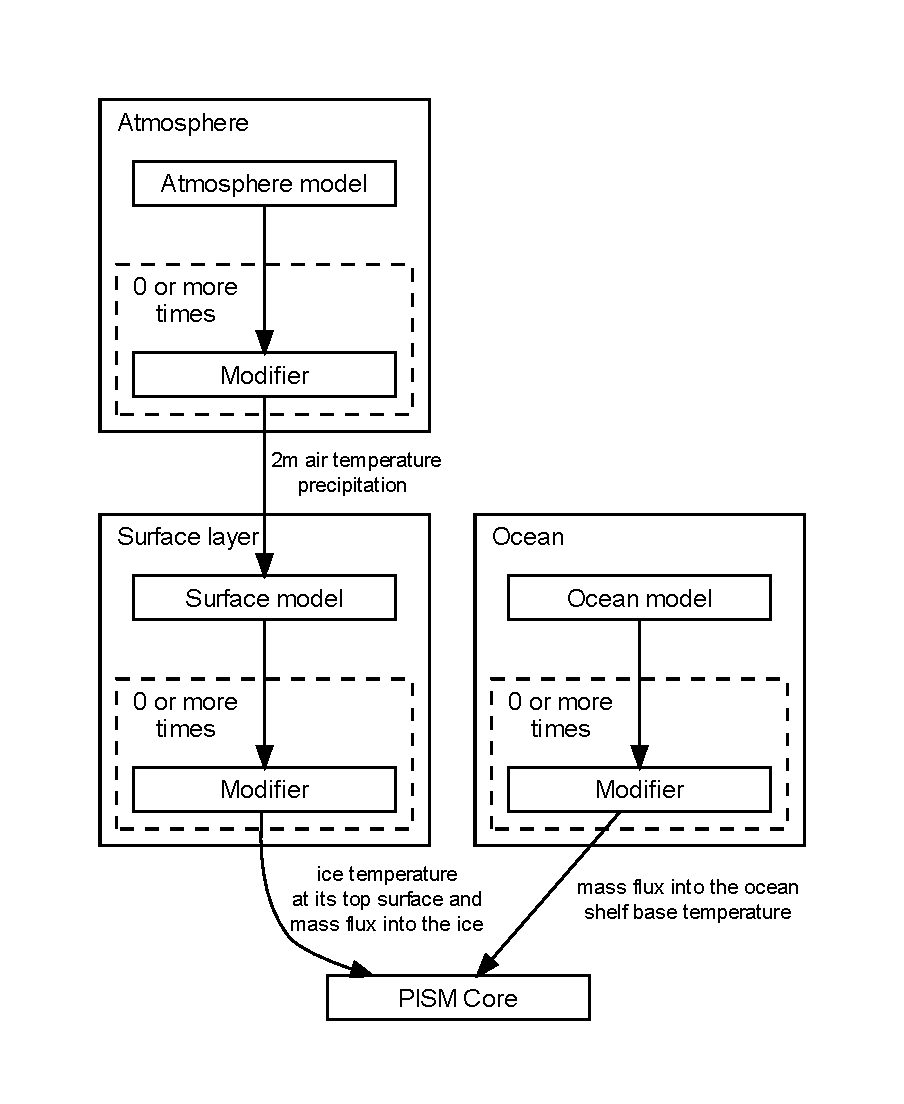
\includegraphics[height=5in]{figs/data-flow.pdf}
  \caption{PISM climate input data flow.}
  \label{fig:climate-input-data-flow}
\end{figure}

\section{Managing model time}
\label{sec:model-time}
\optsection{Managing time}

\subsection{Periodic climate data}
\label{sec:periodic-forcing}

\subsection{Using time bounds in forcing data}
\label{sec:time-bounds}

\subsection{Calendars}
\label{sec:calendars}
Internally PISM stores time in seconds since a specified moment in time and
does not use or need a calendar.

XX-century and prognostic runs require knowledge of lengths of months and
years, both to use climate data properly and to facilitate model validation
using observations.

The following sections describe two modes of time management implemented in
PISM.

\subsubsection{\texttt{365_day} calendar}
\label{sec:365-day}

The default \texttt{365_day} calendar is the default and is used in all PISM
runs that do not require precise application of forcing data or reporting on
particular dates.

\subsubsection{\texttt{gregorian} calendar}
\label{sec:gregorian}

The command-line option \txtopt{calendar}{\texttt{gregorian}} enables the Gregorian
calendar mode.

There are two major consequences:
\begin{itemize}
\item PISM uses the date in\texttt{units} attributes of coordinate variables in
  unit conversions. Please make sure that the \texttt{time} variable in all
  forcing files has the units attribute such as ``\texttt{days since
    2012-1-1}''. PISM will stop with an error message if a time variable does
  not have a reference date in its unit specification.

  Please use units that are a fixed multiple of ``seconds'', such as
  ``\texttt{minutes since 1989-1-1}'' or ``\texttt{days since 1999-12-31}'' and
  avoid ``months'' and ``years''. (PISM uses UDUNITS-2 to convert units, and in
  UDUNITS $1\, \mathrm{month} = \frac{1}{12}\cdot 365.2524\, \mathrm{days}$.)
\item PISM uses dates in standard output:
\begin{verbatim}
...
   time interval (length)   [2012-01-01, 2021-12-31]  (10.000 years)
...
S 2012-05-26:  0.00011    0.6306   0.00000000           0.00000
$v$Eh m (dt=0.10000)
S 2012-07-01:  0.00014    0.6306   0.00000000           0.00000
\end{verbatim}
\end{itemize}

Just like in the \texttt{365_day} mode, run length, run start and run end times
are specified using \intextoption{y}, \intextoption{ys} and \intextoption{ye}
command-line options, respectively. Note that here \texttt{-y 1} has the
meaning of $3.14...\cdot 10^{7}$ seconds (one ``tropical year''), \emph{not} a
calendar year.

To specify the reference date, i.e. the date corresponding to time $0$, use the
\txtopt{reference_date}{\texttt{YYYY-MM-DD}} command-line option or the
\texttt{reference_date} configuration parameter.

For example, to run for $20$ years starting in $1989$ and override time read
from an input file, do
\begin{verbatim}
$ pismr -calendar gregorian -reference_date 1989-1-1 -ys 0 -ye 20
\end{verbatim}

It is also possible to run PISM for the duration of the available forcing data:
\begin{verbatim}
$ pismr -calendar gregorian -time_file forcing.nc
\end{verbatim}
will extract the reference date and run length from \texttt{forcing.nc}
(respecting time bounds).

It is also possible to save spatial and/or scalar time-series daily, monthly or
yearly (using the Gregorian calendar). See sections \ref*{userman-sec:saving-time-series}
and \ref*{userman-sec:saving-spat-vari} of the User's Manual.

\section{Known use cases}
\label{sec:known-use-cases}

\subsection{Using forcing provided by a regional climate model}
\label{sec:regional-model}

\subsubsection{Ice surface temperature and mass balance}
\label{sec:ice-surface-bc}

\subsubsection{Air temperature and precipitation}
\label{sec:air-temp-and-precip}


\subsection{Using climate anomalies}
\label{sec:climate-anomalies}


\subsection{Paleo-climate runs}
\label{sec:paleo-climate}

\section{Checking if forcing data is used correctly}
\label{sec:checking-forcing}


\subsection{Visualizing climate inputs, without ice dynamics}
\label{sec:pclimate}
\optsection{\texttt{pclimate} options}

Recall that internally in PISM there is a separation of climate inputs from ice
dynamics (subsection \ref{sec:climate-inputs}). Executable
\texttt{pclimate} \index{executables!\texttt{pclimate}} allows one to visualize climate inputs without
invoking the ice dynamics core of PISM. This is helpful during the process of
creating PISM-readable data files, and modeling with such.

\texttt{pclimate} shares the code implementing climate models with other PISM
executables, so everything said in section \ref{sec:boundary-models} applies
here. In addition to \texttt{-atmosphere}, \texttt{-surface}, \texttt{-ocean}
and others, \texttt{pclimate} takes options listed in table \ref{tab:pclimate}.

\begin{table}[ht]
  \centering
  \caption{\texttt{pclimate} command-line options}
  \begin{tabular}{p{0.25\linewidth}p{0.7\linewidth}}\toprule
    \textbf{Option} & \textbf{Description}\\
    \midrule
    \fileopt{i} & specifies an input file, which has been produced by PISM;\\
    \fileopt{o} & sets the output file name;\\
    \txtopt{ys}{(years)} & sets the start time, in years;\\
    \txtopt{ye}{(years)} & sets the final time, in years;\\
    \txtopt{dt}{(years)} & sets the interval between saved climate snapshots.\\
    \bottomrule
 \end{tabular}
 \label{tab:pclimate}
\end{table}

\bigskip
As an example, set up an ice sheet state file and run \texttt{pclimate} on it:
\begin{verbatim}
$ mpiexec -n 2 pisms -eisII A -y 1000 -o state.nc
$ pclimate -i state.nc -surface constant -ys 0.0 -ye 2.5 -dt 0.1 -o movie.nc
\end{verbatim}
Using \texttt{pisms} merely generates demonstration climate data, using
EISMINT II choices \cite{EISMINT00}.  \texttt{pclimate} extracts the 
surface mass balance \texttt{acab} and surface temperature \texttt{artm} from \texttt{state.nc}.
It then does nothing interesting, exactly because a constant climate
is used.  Viewing \texttt{movie.nc} we see these same values as from \texttt{state.nc},
in variables \texttt{acab}, \texttt{artm}, reported back to us as the time- and space-dependent
climate at times \texttt{ys:dt:ye}.  It is a boring ``movie.''

The excuse for the executable \texttt{pclimate} becomes clearer if we use a positive degree-day
model (subsection \ref{sec:boundary-models}).  The positive degree-day
model uses a variable called \texttt{precip}, and a calculation of melting, to get the
surface mass balance \texttt{acab}. 

Assuming that \texttt{g20km_pre100.nc} was created as described in section
\ref{sect:start}, running
\begin{verbatim}
$ pclimate -i g20km_pre100.nc -atmosphere searise_greenland \
           -surface pdd -ys 0 -ye 2.5 -dt 0.1 -o foo.nc
\end{verbatim}%$
produces \texttt{foo.nc}. Viewing in with \texttt{ncview} shows an annual cycle
in the variable \texttt{airtemp} and a noticeable decrease in the surface mass
balance during summer months (see variable \texttt{acab}). Note that
\texttt{artm} is constant in time: this is the temperature \emph{at the ice
  surface but below firn} and it does not include seasonal variations \cite{Hock05}.

See section \ref{sec:eismint-greenland} for another \texttt{pclimate} example.

\subsection{Low-resolution test runs}
\label{sec:low-resolution-test-runs}

\section{Atmosphere models}
\label{sec:atmosphere}
\optsection{Climate (boundary) models!\texttt{-atmosphere} [searise_greenland, constant, given, lapse_rate, forcing]}

\subsection{SeaRISE-Greenland}

Option: \texttt{searise_greenland}

This atmosphere model implements a longitude, latitude and elevation dependent near-surface air temperature parameterization and a cosine yearly cycle described in \cite{Faustoetal2009} and uses a constant in time ice-equivalent precipitation field (in units of thickness per time, variable \texttt{precip}) that is read from an input file.  The air temperature parameterization is controlled by configuration parameters with the \texttt{snow_temp_fausto} prefix.

In addition to the temperature parameterization it allows using the SeaRISE-Greenland formula for paleo-precipitation correction from present; a 7.3\% change of precipitation rate for every one degree Celsius of temperature change \cite{Huybrechts02}.  See \url{http://websrv.cs.umt.edu/isis/index.php/Model_Initialization#Greenland} for details.  Turn on this mechanism by using the \intextoption{paleo_precip} option.

It expects variables \texttt{precip}, latitude and longitude to be present in an input file.

\subsection{Constant in time}
\label{sec:constant-time}

Option: (\texttt{constant})

This atmosphere model reads the snow precipitation (variable \texttt{precip}) and the mean annual near-surface air temperature (variable \texttt{artm}) and provides them to a surface model.

\subsection{Reading atmosphere boundary conditions from a file}
\label{sec:read-atmosph-bound}

(\texttt{given})

This atmosphere model is similar to \texttt{constant} in that it uses \texttt{artm} and \texttt{precip} fields given by the user by providing them directly to the surface model. The name of the file PISM will read \texttt{artm} and \texttt{precip} from is specified using the \fileopt{atmosphere_given_file} option.

A file \texttt{foo.nc} used with \texttt{-atmosphere given -atmosphere_given_file foo.nc} should contain several records;\footnote{If this file contains one record (i.e. fields corresponding to one time value only), \texttt{-atmosphere given} is essentially equivalent to \texttt{-atmosphere constant}.} the time variable (\texttt{'t'}) should describe what model time these records correspond to.

This model was created to force PISM with sampled (possibly periodic) climate data, e.g. using monthly records of \texttt{artm} and \texttt{precip}.


Currently there are two ``modifiers'' one can use with an atmosphere model.

The atmosphere \texttt{dTforcing} modifier implements temperature forcing using scalar offsets and \texttt{anomaly} modifier a mechanism applying precipitation and temperature anomalies.
\begin{itemize}
\item \fileopt{dTforcing} specifies a file containing scalar temperature
  offsets (for use with \texttt{dTforcing}, variable \texttt{delta_T}),
\item \fileopt{anomaly_temp} specifies a file containing spatially-variable
  near-surface air temperature anomalies (variable \texttt{temp_anomaly}),
  and
\item \fileopt{anomaly_precip} specifies a file containing spatially-variable
  ice-equivalent precipitation anomalies (in units of thickness per time,
  variable \texttt{precip_anomaly}).
\end{itemize}

Options \texttt{-anomaly_temp} and \texttt{-anomaly_precip} can be used to
set up a PISM run using a GCM output, essentially achieving one-way coupling.
See also the \texttt{-surface given} option, below.

The \texttt{lapse_rate} modifier allows correcting air temperature and
precipitation using elevation lapse rates. It uses the following options.
\begin{itemize}
\item \fileopt{atmosphere_given_file} specifies the file containing the
  reference surface elevation field (standard name:
  \texttt{surface_altitude}). This file can contain several surface elevation
  records to use lapse rate corrections relative to time-dependent surface.
  If one record is provided, the reference surface elevation is assumed to be
  time-independent.
\item \intextoption{atmosphere_given_period} gives the period, in model
  years, to use when interpreting data in the file given with
  \texttt{-atmosphere_given_file},
\item \intextoption{atmosphere_given_reference_year} takes the time $T$ in
  model years. The record for $t$ years in \texttt{-atmosphere_given_file} is
  interpreted as corresponding to $t$ years since $T$.
\item \intextoption{atmosphere_given_time_average} enables interpolating (and
  in some cases, averaging) B.C. data in time.
\item \intextoption{temp_lapse_rate} gives the temperature lapse rate, in
  $K/km$. Note that we use the following definition of the temperature lapse
  rate:
  \begin{displaymath}
    \gamma = -\frac{dT}{dz}.
  \end{displaymath}
\item \intextoption{precip_lapse_rate} gives the precipitation lapse rate, in
  $m/year/km$. Here $\gamma = -\frac{dM}{dz}$.
\end{itemize}

\subsection{EISMINT-Greenland}
\label{sec:eismint-greenland}

\subsection{PIK}
\label{sec:atmosphere-pik}


\section{Atmosphere model modifiers}
\label{sec:atmosphere-mods}

\subsection{Scalar temperature offsets}
\label{sec:delta-temp}

\subsection{Scalar precipitation offsets}
\label{sec:delta-precip}

\subsection{Lapse rate corrections}
\label{sec:lapse-rates}

\subsection{Anomalies}
\label{sec:anomalies}



\section{Surface mass and energy process models}
\label{sec:surface-snow}
\optsection{Climate (boundary) models!\texttt{-surface} [simple, constant, elevation, given, pdd, forcing]}

\subsection{The ``invisible'' model}
\label{sec:invisible-model}

(\texttt{simple}, the default)

This is the simplest ``surface model'' available in PISM. Its job is to
re-interpret precipitation as surface mass flux (balance), and to re-interprets
mean annual near-surface (2m) air temperature as the temperature of the ice at
the depth at which firn processes cease to change the temperature of the ice.
(I.e.~the temperature \emph{below} the firn.) This implies that there is no
melt. Though primitive, this model may be desired in cold environments
(e.g.~East Antarctic ice sheet) in which melt is negligible and heat from firn
processes is ignored.

\subsection{Constant in time}
\label{sec:constant-time-1}

(\texttt{constant})

This surface model reads constant in time ice upper surface boundary conditions
from a file. These fields are provided directly to the ice dynamics model (see
table \ref{tab:ice-dynamics-bc}). Variables \texttt{artm} (ice temperature at
the ice surface but below firn) and \texttt{acab} (top surface mass flux into
the ice) are read from the file, so this choice will cause PISM to stop if they
are not present in the input file.

Note: this surface model \emph{ignores} the atmosphere model selection made
using the \texttt{-atmosphere} option.

\subsection{Reading top-surface boundary conditions from a file}
\label{sec:reading-top-surface}

(\texttt{given})

This surface model is similar to \texttt{constant} in that it uses \texttt{artm} and \texttt{acab} fields given by the user by providing them directly to the ice dynamics model. The name of the file PISM will read \texttt{artm} and \texttt{acab} from is specified using the \fileopt{surface_given_file} option.

A file \texttt{foo.nc} used with \texttt{-surface given -surface_given_file foo.nc} should contain several records;\footnote{If this file contains one record (i.e. fields corresponding to one time value only), \texttt{-surface given} is essentially equivalent to \texttt{-surface constant}.} the time variable (\texttt{'t'}) should describe what model time these records correspond to.

This model was created to force PISM with sampled (possibly periodic) climate data, e.g. using monthly records of \texttt{artm} and \texttt{acab}.

Option \txtopt{surface_given_period}{years} makes PISM interpret data in \texttt{-surface_given_file} as periodic. In this case the time in the NetCDF file is understood as the time \emph{from the beginning of a period}, i.e. from the beginning of a year with \texttt{-surface_given_period 1}, from the beginning of a decade with \texttt{-surface_given_period 10}, etc.

For example, to use monthly records and period of 1 year, create a file (say, ``\texttt{foo.nc}'') with 12 records. The variable \texttt{'t'} should contain 0, 1, 2, 3, \dots, 11 and have the units of ``month'' (you can use other units, too). Then, run
\begin{verbatim}
$ pimsr -surface given -surface_given_file foo.nc -surface_given_period 1
\end{verbatim}%$

To force PISM using monthly records with longer periods, just add more records to the \texttt{-surface_given_file}  and change the \texttt{-surface_given_period} value.

\noindent Notes:
\begin{itemize}
\item PISM can handle files with virtually any number of records: it will
  read and store in memory at most \texttt{climate_forcing_buffer_size} records
  at any given time (default: 60, or 5 years' worth of monthly fields).
\item this surface model \emph{ignores} the atmosphere model selection made
  using the \texttt{-atmosphere} option,
\item when preparing a file for use with this model, it is best to use the \texttt{t,x,y} variable storage order: files using this order can be read in faster than ones using the \texttt{t,y,x} order, for reasons explained in section \ref{sec:pism-io-performance}.

  To change the storage order in a NetCDF file, use \texttt{ncpdq}:
\begin{verbatim}
$ ncpdq -a t,x,y input.nc output.nc
\end{verbatim}%$
  will copy data from \texttt{input.nc} into \texttt{output.nc}, changing the storage order to \texttt{t,x,y} at the same time.
\end{itemize}

\subsection{Elevation-dependent temperature and mass balance}
\label{sec:elev-depend-temp}

(\texttt{elevation})

This surface model parametrizes the ice surface temperature $T_{h}$ = \texttt{artm} and the surface mass balance $m$ = \texttt{acab} as a \emph{piecewise-linear} function of surface elevation $h$.

The option \txtopt{artm}{\emph{list of 4 numbers}} determines the surface temperature using the 4 parameters $T_{\mathrm{min}}$, $T_{\mathrm{max}}$, $h_{\mathrm{min}}$, $h_{\mathrm{max}}$. Let
\begin{equation}
  \mathrm{d}T/\mathrm{d}h = (T_{\text{max}} - T_{\text{min}}) / (h_{\text{max}} - h_{\text{min}})
\end{equation}
be the temperature gradient.  Then
\begin{equation}
  T(x,y) = \begin{cases}
    T_{\text{min}}, & h(x,y) \le h_{\text{min}}, \\
    T_{\text{min}} + \mathrm{d}T/\mathrm{d}h\,(h(x,y) - h_{\text{min}}),
    &  h_{\text{min}} < h(x,y) < h_{\text{max}}, \\
    T_{\text{max}}, & h_{\text{max}} \le h(x,y). \end{cases}
\end{equation}

The option \txtopt{acab}{\emph{list of 5 numbers}} determines the surface mass balance using the 5 parameters $m_{\mathrm{min}}$, $m_{\mathrm{max}}$, $h_{\mathrm{min}}$, $h_{\mathrm{ELA}}$, $h_{\mathrm{max}}$. Let
\begin{equation}
  \mathrm{d}m_{\mathrm{abl}}/\mathrm{d}h = - m_{\text{min}} / (h_{\text{max}} - h_{\text{min}})
\end{equation}
and
\begin{equation}
  \mathrm{d}m_{\mathrm{acl}}/\mathrm{d}h = m_{\text{max}} / (h_{\text{max}} - h_{\text{min}})
\end{equation}
be the mass balance gradient in the ablation and in the accumulation area, respectively.  Then
\begin{equation}
  m(x,y) = \begin{cases}
    m_{\text{min}}, & h(x,y) \le h_{\text{min}}, \\
    \mathrm{d}m_{\mathrm{abl}}/\mathrm{d}h\,(h(x,y) - h_{\text{ELA}}),
    &  h_{\text{min}} < h(x,y) < h_{\text{max}}, \\
    \mathrm{d}m_{\mathrm{acl}}/\mathrm{d}h\,(h(x,y) - h_{\text{ELA}}),
    &  h_{\text{min}} < h(x,y) < h_{\text{max}}, \\
    m_{\text{max}}, & h_{\text{max}} \le h(x,y). \end{cases}
\end{equation}
The option \txtopt{acab_limits}{\emph{list of 2 numbers}} limits the mass balance below $h_{\mathrm{min}}$ to $m^{*}_{\mathrm{min}}$ and above $h_{\mathrm{max}}$ to $m^{*}_{\mathrm{max}}$, thus
\begin{equation}
  m(x,y) = \begin{cases}
    m^{*}_{\text{min}}, & h(x,y) \le h_{\text{min}}, \\
    \mathrm{d}m_{\mathrm{abl}}/\mathrm{d}h\,(h(x,y) - h_{\text{ELA}}),
    &  h_{\text{min}} < h(x,y) < h_{\text{max}}, \\
    \mathrm{d}m_{\mathrm{acl}}/\mathrm{d}h\,(h(x,y) - h_{\text{ELA}}),
    &  h_{\text{min}} < h(x,y) < h_{\text{max}}, \\
    m^{*}_{\text{max}}, & h_{\text{max}} \le h(x,y). \end{cases}
\end{equation}

Note: this surface model \emph{ignores} the atmosphere model selection made using the \texttt{-atmosphere} option.

\subsection{Temperature-index (positive degree-day) scheme}
\label{sec:temp-index-posit}

(\texttt{pdd}) \index{temperature-index surface processes model} \index{positive degree day surface processes model} \index{PDD (positive degree day model)} \index{PISM!default positive degree day model} 

The default PDD used by PISM, turned on by option \texttt{-surface pdd}, is
based on \cite{CalovGreve05} and EISMINT-Greenland intercomparison (section
\ref{sec:eismint-greenland} and \cite{RitzEISMINT}).

Our PDD implementation is meant to be used with an atmosphere model
implementing a cosine yearly cycle such as \texttt{searise_greenland} and
\texttt{eismint_greenland}, but is not restricted to parameterizations like
this one. A PDD generally adds ``white noise'' to the seasonal cycle to
simulate additional daily variability associated to the vagaries of weather.
This additional random variation is quite significant, as the seasonal cycle
may never reach the melting point but that point may be reached with some
probability, in the presence of the daily variability, and thus melt may occur.
Concretely, a normally-distributed, mean zero random temperature increment is
added to the seasonal cycle. There is no assumed spatial correlation of daily
variability. The standard deviation of the daily variability is controlled by
the \intextoption{pdd_std_dev} option, and the corresponding configuration
parameter has the same name. The default value is 5.0 degrees
\cite{RitzEISMINT}.

The number of positive degree days is computed as the magnitude of the
temperature excursion above $0\!\phantom{|}^\circ \text{C}$ multiplied by the
duration (in days) when it is above zero. In PISM there are actually two
methods for computing the number of positive degree days. The first computes
only the expected value, by the method described in \cite{CalovGreve05}. This
is the default when a PDD is chosen (i.e.~option \texttt{-surface pdd}). The
second is a monte carlo simulation of the white noise itself, chosen by adding
the option \intextoption{pdd_rand}. This monte carlo simulation adds the same
daily variation at every point, though the seasonal cycle is (generally)
location dependent. If repeatable randomness is desired use
\intextoption{pdd_rand_repeatable} instead of \texttt{-pdd_rand}.

The number of positive degree days is multiplied by a coefficient (config
parameter \texttt{pdd_factor_snow}) to compute the amount of snow melted. Of
the melted snow, a fraction (\texttt{pdd_refreeze}) is kept as ice. This ice,
plus all unmelted snow (already measured as ice-equivalent) is added to the
mass balance, unless the number of positive degree days exceeds that required
to melt all of the snow. In this latter case, in which there are excess
positive degree days available for melting, the excess is multiplied by a
coefficient (\texttt{pdd_factor_ice}) to compute how much ice is melted. In
this case actual ablation occurs at that location.

In addition to this, one may use latitude- and July-air-temperature-dependent
Greenland PDD model parameters $\beta_{\mathrm{ice}}$ and
$\beta_{\mathrm{snow}}$ (formulas (6) and (7) in \cite{Faustoetal2009}) by
adding the \intextoption{pdd_fausto} option. It also implements latitude- and
mean July temperature dependent ice and snow factors using formulas in
\cite{Faustoetal2009}. The standard deviation of the daily variability
(\intextoption{pdd_std_dev} option) is 2.53 degrees under the
\intextoption{pdd_fausto} option \cite{Faustoetal2009}. See also configuration
parameters with the \texttt{pdd_fausto} prefix.

\subsection{PIK}
\label{sec:surface-pik}


\section{Surface model modifiers}
\label{sec:modifiers}

\subsection{Scalar temperature offsets}
\label{sec:surface-delta-temp}

The \texttt{dTforcing} modifier implements temperature forcing using scalar
offsets and uses the \texttt{-dTforcing} option. This modifier is identical to
the corresponding atmosphere modifier, but applies offsets at a different stage
in the computation of top-surface boundary conditions needed by the ice
dynamics core.

\subsection{Temperature and mass balance anomalies}
\label{sec:temp-smb-anomalies}



\subsection{Lapse rate corrections}
\label{sec:surface-lapse-rates}

The \texttt{lapse_rate} modifier allows correcting ice-surface temperature and
surface mass balance using elevation lapse rates. It uses the following
options.

\begin{itemize}
\item \fileopt{surface_given_file} specifies the file containing the reference
  surface elevation field (standard name: \texttt{surface_altitude}). This file
  can contain several surface elevation records to use lapse rate corrections
  relative to time-dependent surface. If one record is provided, the reference
  surface elevation is assumed to be time-independent.
\item \intextoption{surface_given_period} gives the period, in model years, to
  use when interpreting data in the file given with
  \texttt{-surface_given_file},
\item \intextoption{surface_given_reference_year} takes the time $T$ in model
  years. The record for $t$ years in \texttt{-surface_given_file} is
  interpreted as corresponding to $t$ years since $T$.
\item \intextoption{surface_given_time_average} enables interpolating (and in
  some cases, averaging) B.C. data in time.
\item \intextoption{temp_lapse_rate} gives the temperature lapse rate, in
  $K/km$. Note that we use the following definition of the temperature lapse
  rate:
  \begin{displaymath}
    \gamma = -\frac{dT}{dz}.
  \end{displaymath}
\item \intextoption{smb_lapse_rate} gives the surface mass balance lapse rate,
  in $m/year/km$. Here, $\gamma=-\frac{dM}{dz}$.
\end{itemize}

\subsection{Surface mass flux adjustment}
\label{sec:smb-adjustment}

The \texttt{forcing} modifier implements a surface mass balance adjustment
mechanism which forces ice thickness to a target thickness distribution at the
end of the run. The idea behind this mechanism is that spinup of ice sheet
models frequently requires the surface elevation to come close to measured
values at the end of a run. A simpler alternative to accomplish this, namely
option \intextoption{no_mass}, represents an unmodeled, frequently large,
violation of the mass continuity equation.

In more detail, let $H_{\text{tar}}$ be the target thickness. Let $H$ be the
time-dependent model thickness. Note that a surface model as described in this
section produces the $M$ term in the mass continuity equation
$$\frac{\partial H}{\partial t} = M - S - \nabla\cdot \mathbf{q}.$$
(Other details of this equation do not concern us here.) Option
\fileopt{force_to_thk} causes $M$ to be modified by a multiple of the
difference between the target thickness and the current thickness,
$$\Delta M = \alpha (H_{\text{tar}} - H)$$
where $\alpha>0$. We are adding mass ($\Delta M>0$) where $H_{\text{tar}} > H$
and ablating where $H_{\text{tar}} < H$. We make this mechanism stronger as the
run goes on, as follows: if $t_s$ be the start time and $t_e$ the end time for
the run then $\alpha=\alpha(t)$ where $\alpha(t) = \alpha_0 (t-t_s)/(t_e-t_s)$.

Option \fileopt{force_to_thk} identifies the file containing the target ice
thickness field. A basic run modifying surface model \texttt{constant} would
look like
\begin{verbatim}
$ pismr -i foo.nc -surface constant,forcing -force_to_thk bar.nc
\end{verbatim}%$

In this case \texttt{foo.nc} contains fields \texttt{acab} and \texttt{artm},
as normal for \texttt{-surface constant}, and \texttt{bar.nc} contains field
\texttt{thk} which will serve as the target thickness. Option
\intextoption{force_to_thk_alpha} adjusts the value of $\alpha_0$, which has a
default value specified in the \emph{Source Code Browser}
\url{\PISMBROWSERURL}.






\section{Ocean models}
\label{sec:pism-ocean-models}
\optsection{Climate (boundary) models!\texttt{-ocean} [constant, forcing]}

PISM includes one simple ocean model: \texttt{constant}, providing constant
(both in time and space) mass flux into the ocean and sea level elevation to
PISM's ice flow core. The mass flux is controlled by the\\
\texttt{ocean_sub_shelf_heat_flux_into_ice} configuration parameter and the
assumption that the mass flux is proportional to heat flux into ice.
Alternatively, the sub shelf basal melt rate in meters ice-equivalent per year
can be set at the command-line with \intextoption{shelf_base_melt_rate}.

The ocean \texttt{dSLforcing} modifier implements sea level forcing. The
command-line option \fileopt{dSLforcing} is used to specify the file containing
sea level offsets:
\begin{verbatim}
$ pismr -i in.nc -ocean constant,dSLforcing -dSLforcing delta_SL.nc
\end{verbatim}%$
uses \texttt{delta_SL.nc}

\subsection{Constant in time}
\label{sec:constant-time-2}

\subsection{Reading forcing data from a file}
\label{sec:ocean-given}

\subsection{PIK}
\label{sec:ocean-pik}

\section{Ocean model modifiers}
\label{sec:ocean-mods}

\subsection{Scalar sea level offsets}
\label{sec:delta-sea-level}

\subsection{Scalar sub-shelf temperature offsets}
\label{sec:delta-subshelf-temp}

\subsection{Scalar sub-shelf mass flux offsets}
\label{sec:delta-subshelf-smb}



% References and indices
\clearpage\newpage
\bibliography{ice-bib}
\bibliographystyle{siam}

\phantomsection
\addcontentsline{toc}{section}{General Index}
\label{sect:index}
\printindex

\phantomsection
\addcontentsline{toc}{section}{PISM Command-line options}
\printindex[options]

\end{document}
